\subsection{Handling ``fast'' cards}
	

\begin{figure}[htp]
\begin{center}
  \includegraphics[width=0.4\textwidth]{pics/sdmBilder/bindings/fastcard}
  \caption{Fast cards are a special kind of card.}  
  \label{fig:sdm_fastcard_1}
\end{center}
\end{figure}

\begin{figure}[htp]
\begin{center}
  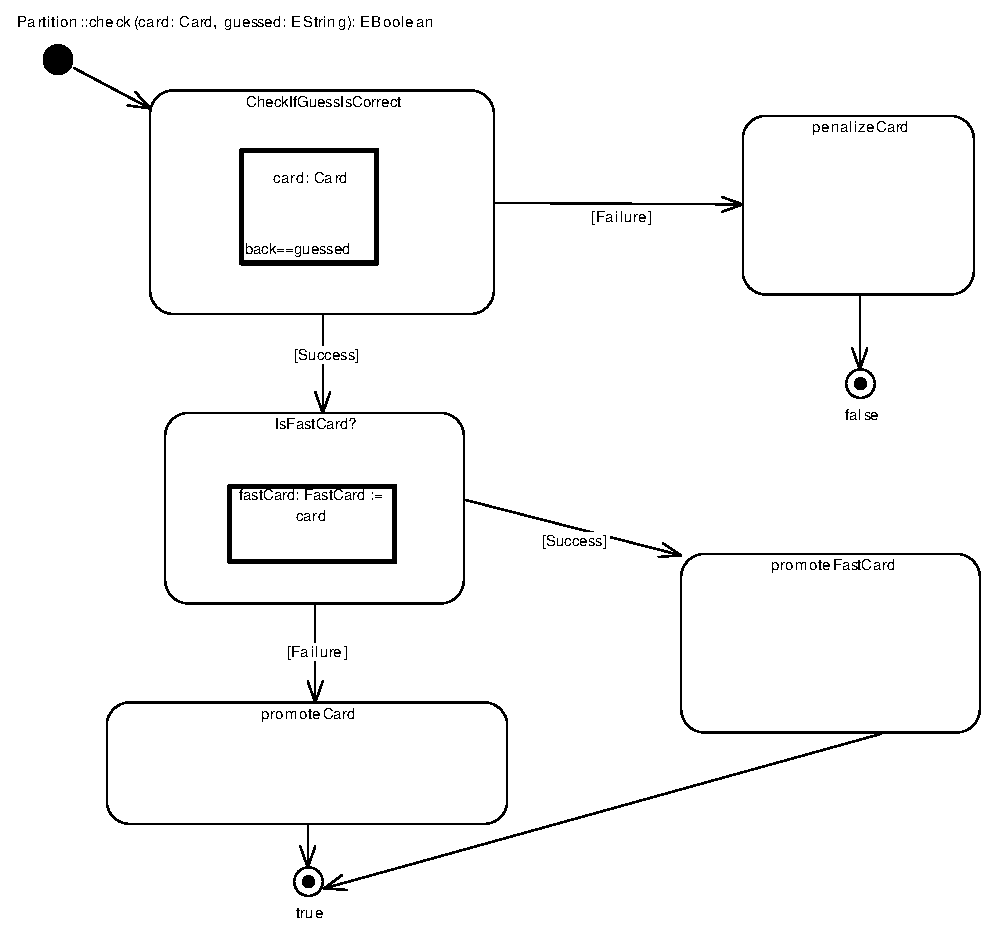
\includegraphics[width=0.5\textwidth]{pics/sdmBilder/bindings/fastcard_controlflow}
  \caption{Extend check to handle fast cards.}  
  \label{fig:sdm_fastcard_2}
\end{center}
\end{figure}

\begin{figure}[htp]
\begin{center}
  \includegraphics[width=0.5\textwidth]{pics/sdmBilder/bindings/fastcard_bindingexp}
  \caption{Create a binding for \texttt{fastcard}.}  
  \label{fig:sdm_fastcard_3}
\end{center}
\end{figure}

\begin{figure}[htp]
\begin{center}
  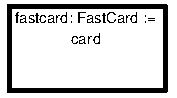
\includegraphics[width=0.2\textwidth]{pics/sdmBilder/bindings/visual_bindingexp}
  \caption{Visualisation for binding expression.}  
  \label{fig:sdm_fastcard_4}
\end{center}
\end{figure}

\begin{figure}[htp]
\begin{center}
  \includegraphics[width=0.8\textwidth]{pics/sdmBilder/bindings/promoteFastCard}
  \caption{Story pattern for handling fast cards.}  
  \label{fig:sdm_fastcard_5}
\end{center}
\end{figure}




